% !Mode:: "TeX:UTF-8"

\BiChapter{密集热点区域无线网络的性能分析}{Performace Analysis}

论文的第二章已经介绍了密集热点区域无线网络的定义,根据密集热点区域无线网络的定义,我们就可以构造密集热点区域无线网络的网络模型。
构造密集热点区域无线网络的模型需要从四个方面考虑,即基站的拓扑结构,用户统计分布,信道建模与网络架构建模。在本章中,主要考虑前三个方面。

在第三章,通过对密集热点区域无线网络的系统建模,即可对密集热点区域无线网络的下行链路进行分析。通过性能分析,我们可以得到用户的信干比,网络的覆盖率,网络的单位面积频谱利用率等性能指标。

在第四章,着重考虑密集热点区域无线网络的网络架构,对密集热点区域无线网络的性能进行优化,引入提出的资源管理和调度算法,网络的覆盖率,服务用户数,单位面积频谱利用率,单位面积能量谱利用率将进一步提高。


\BiSection{密集热点区域无线网络的系统建模}{System Model}
本小节对密集热点区域无线网络进行系统建模,主要包括基站的参数与拓扑结构的分析与建模,用户的在服务区内的统计特性建模以及信道建模。
本论文主要考虑单小区,小区中配备有多个微基站。
本论文主要对下行链路的性能进行分析,即信源在基站侧,在基站中完成调制、编码发送等信号处理过程,经过信道传送至用户侧,用户在进行接收、解调、解码等过程将信息接收。
宏基站和微基站采用不同的频谱资源。
假设小区为的区域面积为~$A$。用户与发射基站建立的链路受到大尺度衰落的影响,路径损耗系数为~$\alpha$,信道噪声为加性高斯白噪声,噪声的功率为~$N$,
信道类型为瑞利信道,信道系数~$h$~服从单位指数分布,记做~$h\sim exp(1)$。$h$~的概率密度分布函数为:
\begin{equation}\label{h_pdf}
  f_H(h) = \exp(-h)
\end{equation}
概率累计分布函数为:
\begin{equation}\label{h_cdf}
  F_H(h) = \mathbb{P}[H\leq h] = 1 - \exp(-h)
\end{equation}

用户选择距离自己最近的微基站作为服务基站。
\BiSubsection{基站的参数与拓扑结构}{topology}

为了便于以后的性能分析,需要根据之前对超密集组网定义的描述,对基站的参数指标进行说明。

假设微基站的发射功率为~$P$~、每个基站配备有单根天线,小区中有多个微基站,微基站的个数为~$n$~,小区中微基站的密度为~$\lambda$~,小区密度和小区基站之间的关系如~(\ref{bs_dens_num})~所示:
\begin{equation}\label{bs_dens_num}
  n_s = \biggl\lfloor\lambda_s S\biggr\rfloor
\end{equation}
其中~$\biggl\lfloor\cdot\biggr\rfloor$~表示向下取整。所有微基站构成的集合为~$\mathcal{S}$~,第~$i$~个微基站的编号为~$S_i$~,即~$\mathcal{S}=\left\{S_1, S_2,\dots,S_{n_s}\right\}$。
微基站~$S_i$~服务的用户数为~$k_i$~个。

基站的拓扑结构即为微基站的部署方法微基站的部署则相对灵活,部署方式主要有两种,第一种为传统的格点分布,即在对微基站部署前,需要选定一种格形,如六边形格形,四边形格形等,然后将基站部署在格点上。
第二种为小区中的微基站部署是一个泊松点过程。该方法最先由~J.~ G.~ Andrews~提出\citeup{ATractable},用于刻画地物地貌对基站部署的影响。
将微基站的部署过程考虑为一个泊松点过程是更加合理的,主要有一下三个方面的原因:

(1)~ 基于格形的基站模型过于理想化

由于微基站的密度很高,容易受到外界因素的干扰。
如地形地貌的影响,如果按照格点部署,但是选定的格点周围恰好不适合部署基站,那么格点模型对该区域的刻画就不够准确,就得不到可信的性能分析。
微基站的部署也收附近的用户的统计特性的影响,如果格点周围刚好没有什么用户,显然也不会在格点上部署基站。
此时将网络中的基站建模成为格点分布也是不合理的。

(2)~ 微基站和家庭基站的部署呈现自组织性

在当前的小基站场景下,网络是密集部署的,许多微基站和家庭基站,其部署是自由部署的而不是由运营商统一部署的,这就体现了一定的随机性。
而泊松点过程就是对这种随机性的一种刻画。

(3)~ 方便对网络进行性能分析

将基站的部署看成泊松点过程,就可以应用随机几何中已经得到的很多定理简化分析过程。
通过随机几何这一数学工具,可以简化网络中的信息指标的求解,如覆盖率和单位面积频谱利用率的求解。
而基于格形的基站建模,相关性能参数的精确值只能通过蒙特卡洛仿真得到。

基站部署方式的示意图如图~\ref{bs_dis}~所示:
\begin{figure}[htbp]
\centering
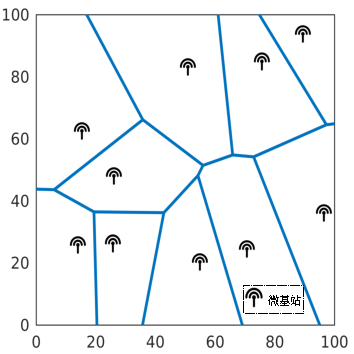
\includegraphics[width = 0.62\textwidth]{bs_dis.pdf}
\caption{基站的拓扑结构示意图}\vspace{-0.5em}
\label{bs_dis}
\end{figure}


从图~\ref{bs_dis}~是密集热点区域无线网络的基站的拓扑结构的示意图,图中,区域大小为~100$\mathrm{m}\times 100\mathrm{m}$~,模拟单个小区的情况,小区中有10个微基站,微基站的密度为~$\lambda=10^{-3}\mathrm{m}^{-2}$。
由于用户选择距离自己最近的基站进行服务,图中也采用Voronoi图对每个基站的服务区域进行了标注,即基站的服务区域为其所属的泰森多边形所占的区域。
如图中描述,微基站的部署是一个泊松点过程~$\phi$,图~\ref{bs_dis}~是泊松点过程的一次实现。
从图中也可以看出,该种基站部署方式的拓扑结构更加符合实际的情况。

当基站的部署过程为泊松点过程时,在直角坐标系下,基站的部署可以近似的看成二维随机分布,即在给定的区域内,基站在每个位置上的概率相同。
同时,根据泊松点过程的性质,已知区域的面积~$A$,那么区域内的微基站的个数~$n$~是一个随机变量,该随机变量服从与面积有关的泊松分布,泊松分布的参数为$\lambda A$。
即:
\begin{equation}
  \mathbb{P}(n_s = i) = \frac{e^{-\lambda A}(\lambda A)^{i}}{i!}
\end{equation}
根据泊松分布的性质,已知区域的面积~$A$~,微基站的密度为~$\lambda$~,则区域内的基站数量的均值为:
\begin{equation}\label{n_s_bar}
  \overline{n_s} = \lambda A
\end{equation}

\BiSubsection{用户终端的统计特性}{user distribution}

超密集组网场景是客观世界中普遍存在的一类场景。
网络区域中人物的活动规律复杂,每个人的容量需求也是十分复杂的。但我们也可以从微基站的部署以及客观实际出发,对小区中用户的统计分布做出合理的假设。

由于微基站服务于热点区域,区域内用户多,用户对容量的需求较高。因此在微基站附近的用户数量和容量需求是远高于宏基站覆盖的其他的范围的。
一般来说,微基站会部署在区域容量需求最高的地方,用户数量和容量需求随着距离微基站的距离越来越远而逐渐的变小。
根据微基站的这一特性,我们引入概率统计学中非常著名的二维混合高斯模型。二维混合高斯模型广泛的应用于人工智能,模式识别,机器学习等领域当中,用于描述事件对行为或决策的影响。
为不是一般性,此处假设二维混合高斯模型的两个维度是相互独立的。

综上所述,对于微基站~$S_i$~,用户的集合为~$\mathcal{U}_i$~,用户的个数为~$k_i$个, 用$U$表示用户的,即~$\mathcal{U}_i=\{U_1, U_2, ..., U_{k_i}\}$~微基站用户的密度为~$\mu$~。
用户围绕着基站服从二维高斯分布,二维高斯分布的方差为~$\sigma^2$。
由于泊松点过程是一个平稳的随机过程,因此可以不是一般性的假设微基站的坐标为原点,则此时,用户的概率密度分布函数即为:
\begin{equation}
  \begin{aligned}
  f_{X,Y}(x,y) &\overset{(a)}{=} f_X(x) f_Y(y) \\
               &\overset{(b)}{=} \frac{1}{\sqrt{2\pi}\sigma}\exp\left(-\frac{x^2}{2\sigma^2}\right)\cdot\frac{1}{\sqrt{2\pi}\sigma}\exp\left(-\frac{y^2}{2\sigma^2}\right) \\
               &=\frac{1}{2\pi\sigma^2}\exp\left(-\frac{x^2+y^2}{2\sigma^2}\right)
  \end{aligned}
\end{equation}

其中~$(a)$~根据随机变量的独立性,~$(b)$~为高斯分布的概率密度函数,X,Y分别为用户的横纵坐标。
用户的分布的概率密度分布函数为如图~\ref{figure_xy_pdf}~所示:
\begin{figure}[htbp]
\centering
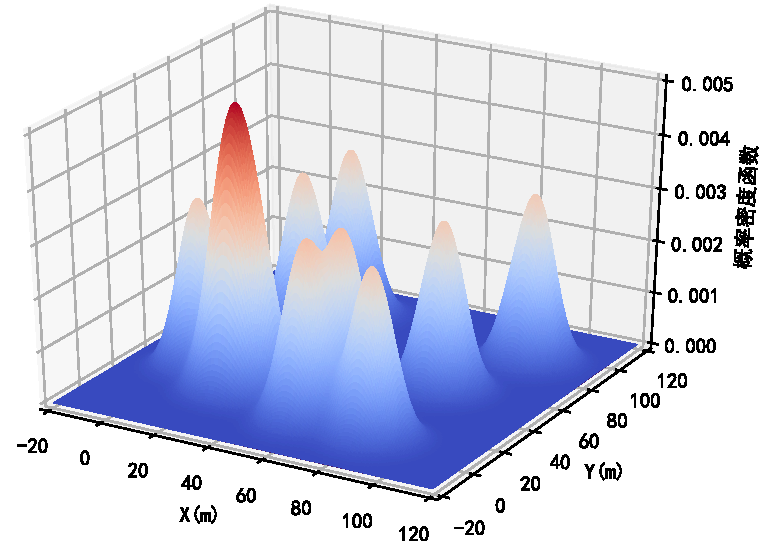
\includegraphics[width = 0.62\textwidth]{figure_xy_pdf.pdf}
\caption{微基站用户的统计分布的概率密度函数}\vspace{-0.5em}
\label{figure_xy_pdf}
\end{figure}

在图中给出了距基站~30m~内的用户的概率密度函数图,其中二维高斯分布的标准差为~10。根据高斯分布的特性,用户多集中在2个标准差范围内,即距离基站的距离为~20m~以内。

可以通过将直角坐标系转换为极坐标系,即可得到用户距基站的距离的概率密度分布函数,分布函数如式~(\ref{r_pdf})~所示:
\begin{equation}\label{r_pdf}
  f_R(r) = \frac{r}{\sigma^2}\exp(-\frac{r^2}{2\sigma^2})
\end{equation}
其中~$R$~为用户距基站的距离。

\BiSection{超密集组网的性能分析}{performance analysis}

本小节对超密集组网场景的模型进行性能分析。主要分析网络的信干噪比,网络的覆盖率以及网络的单位面积频谱利用率。覆盖率和单位面积频谱利用率的概念已在第二章中给出。

小区与用户的参数表总结如下:

\BiSubsection{小区中用户的遍历容量}{SINR}



信干噪比的定义如式~(\ref{SINR})~,可以看出信干噪比是一个与用户的接收功率,用户与服务基站建立的信道上的噪声以及收到其他微基站的干扰功率的和共同决定的。

对于微基站~$S_i$~,其所属的用户~$U_k$~的接收功率用~$P_{i,k}$~表示,如式~(\ref{P_r}):
\begin{equation}\label{P_r}
  P_{i,k} = R_{i,k}^{-\alpha} h_{i,k} P
\end{equation}
其中~$R_{i,k}$~为用户~$U_k$~距基站~$S_i$~的距离,$\alpha$~为信道衰减系数,$h_{i,k}$~是用户~$U_k$~与基站~$S_i$~构成的链路的信道系数,服从单位的指数分布,$h_{i,k}\sim exp(1)$,$P$~为基站的发射功率。
式~(\ref{P_r})~说明用户的接收功率为基站的发送功率经过大尺度衰减和小尺度衰减之后的结果。

微基站~$S_i$~中的用户~$U_k$~会受到其他基站的干扰,同样用户接收到其他基站的功率也是基站的发送功率经过大尺度衰减和小尺度衰减之后的结果,如式~(\ref{I_r})~
\begin{equation}\label{I_r}
  I_{i,k} = \sum_{\begin{subarray}{c} S_j\in \mathcal{S}\\ j \neq i\end{subarray}} R_{j,k}^{-\alpha} h_{j,k} P
\end{equation}
其中~$R_{j,k}$~为用户~$U_k$~距基站~$S_j$~的距离,$\alpha$~为信道衰减系数,$h_{j,k}$~是用户~$U_k$~与基站~$S_j$~构成的链路的信道系数,服从单位的指数分布,$h_{j,k}\sim exp(1)$,$P$~为基站的发射功率。

被微基站~$S_i$~服务的用户~$U_k$~的信干噪比的表达式即为:
\begin{equation}\label{SINR_r}
  \begin{aligned}
    \mathrm{SINR}_{i, k}&\overset{(a)}{=}\frac{P_{i,k}}{I_{i,k}+N} \\
                 &\overset{(b)}{=}\frac{R_{i,k}^{-\alpha} h_{i,k} P}{\sum\limits_{\begin{subarray}{c} S_j\in \mathcal{S}\\ j \neq i\end{subarray}} {R_{j,k}^{-\alpha} h_{j,k} P} + N}
  \end{aligned}
\end{equation}

其中$S_i\in\mathcal{S}$, $U_k\in\mathcal{U}_i$~。$(a)$~为信干噪比的定义,$(b)$~为将式~(\ref{P_r})~和~(\ref{I_r})~带入后的结果。可以看出信干噪比是一个与基站距离,基站的发射功率,噪声,信道衰减系数,信道系数有关的物理量。

由于在超密集组网的场景中,基站与用户之间的距离比较近,因此用户的接收功率在一般情况下是远远大于噪声的,即系统是一个干扰受限的系统。
因此信道的噪声可以忽略不计,忽略后即可得到用户的信干比这一物理量,如式~(\ref{SIR_r})~所示:
\begin{equation}\label{SIR_r}
  \begin{aligned}
    \mathrm{SIR}_{i, k}&\overset{(a)}{=}P_{i,k} / I_{i,k} \\
                 &\overset{(b)}{=}\frac{R_{i,k}^{-\alpha} h_{i,k}}{\sum\limits_{\begin{subarray}{c} S_j\in \mathcal{S}\\ j \neq i\end{subarray}} {R_{j,k}^{-\alpha} h_{j,k}}}
  \end{aligned}
\end{equation}
其中~$(a)$~为信干比的定义,$(b)$~为将式~(\ref{SINR_r})~中忽略噪声之后的结果。

\BiSubsection{小区中用户的覆盖率}{coverage}

覆盖率的定义式为式~(\ref{pc}),由于基站的部署是泊松点过程,泊松点过程是独立平稳的随机过程,因此可以对单个基站的覆盖率进行分析,即可的到网络的覆盖率性能。
因此,不失一般性,可以假设对基站~$S_0\in\mathcal{S}$~进行分析,定义用户距基站~$S_0$~的距离为~$r$,根据前面的分析可知,$r$~服从二维高斯分布,用户与基站~$S_0$~建立的链路的信道系数为~$h$,
$h$~服从单位指数分布,记做~$h\sim exp(1)$。

覆盖率是一个与基站的密度$\lambda$、给定的信干噪比门限~$T$~、信道的衰落系数~$\alpha$、用户的统计分布的参数~$\sigma$~有关系。
可以对式~(\ref{pc})~做进一步的推导。
\begin{equation}\label{pc_expand}
  \begin{aligned}
    p_c(T,~\lambda,~\alpha,~\sigma) &\overset{(a)}{=} \mathbb{P}[\mathrm{SINR}>T] \\
           &\overset{(b)}{=} \mathbb{E}_r[\mathrm{SINR}>T\mid r] \\
           &\overset{(c)}{=} \int_0^\infty \mathbb{P}[\mathrm{SINR}>T\mid r] \frac{r}{\sigma^2}\exp(-\frac{r^2}{2\sigma^2}) \mathrm{d} r
  \end{aligned}
\end{equation}
其中~$T$~为给定的信干噪比的门限,$\lambda$~$(a)$~为覆盖率的定义式,$(b)$~表示网络的覆盖率是一个与距离有关的量,覆盖率的值等于基站中的用户遍历所有可能出现的位置得到的覆盖率的统计平均值,$(c)$~为将式~(\ref{r_pdf})~代入后的结果。

为了得到覆盖率的表达式,需要知道当给定微基站~$S_0$~与用户的距离~$r$~以后信干噪比大于门限的概率,即$\mathbb{P}[\mathrm{SINR}>T]$。
此处假设用户距除~$S_0$~以外最近的基站的距离为~$D$~,则概率可以被拆解成为两个部分。

(1)~ 微基站~$S_0$~的用户恰好被~$S_0$~服务,即用户距基站~$S_0$~的距离~$r < D$。此时,$S_0$~为用户的服务基站,其他基站为干扰基站,即用户受到除~$S_0$~以外的其他基站的干扰。

(2)~ 微基站~$S_0$~的用户被其他的微基站进行服务,即用户距离基站~$S_0$~的距离~$r \geq D$。此时,$S_0$~为干扰基站,即用户受到~$S_0$~基站的干扰,和除服务的微基站以外的其他基站的干扰。

即根据全概率公式,总的覆盖率可以分解为

(1)~ 事件1:所观测用户的服务基站即为所属的热点的基站,且该用户能达到覆盖所需的信干噪比。

(2)~ 事件2:当所观测用户的服务基站为其他基站且该用户能达到覆盖所需的信干噪比。

这两个事件概率的加和。
根据~(1)~和~(2),可以将信干噪比大于门限的概率改写为两个部分,表达式如式~(\ref{P_SINR_2Part})~所示:
\begin{equation}\label{P_SINR_2Part}
  \begin{aligned}
  \mathbb{P}[\mathrm{SINR}>T \mid r] =& \mathbb{P}[\mathrm{SINR}>T \mid r, r < D] \mathbb{P}[r<D]\\
                               &+ \mathbb{P}[\mathrm{SINR}>T \mid r, r > D]\mathbb{P}[r>D]
  \end{aligned}
\end{equation}

对于~$r < D$~的部分,用户受到除了~$S_0$~以外的其他基站的干扰,由于超密集组网系统是一个干扰受限的系统,噪声对系统的影响相比于干扰很小,因此采用信干比,对信干噪比近似。
将信干噪比的表达式~(\ref{SIR_r})~带入到式~(\ref{P_SINR_2Part})~的前半部分,其概率的表达式如式~(\ref{P_SINR_r_le_D})~所示:
\begin{equation}\label{P_SINR_r_le_D}
  \begin{aligned}
  \mathbb{P}[\mathrm{SINR}>T \mid r, r < D] & = \mathbb{P}\left[\frac{r^{-\alpha} h}{\sum\limits_{S_j\in \mathcal{S}\backslash S_0} {R_{j,0}^{-\alpha} h_{0,k}}} > T~\bigg|~ R_{j,0} \geq D > r\right]\\
                                            & = \mathbb{P}\left[h > T r ^ \alpha \sum\limits_{S_j\in \mathcal{S}\backslash S_0} {R_{j,0}^{-\alpha} h_{j,0}}~\bigg|~ R_{j,0} \geq D > r \right]
  \end{aligned}
\end{equation}
为了简化公式,令:
\begin{equation}\label{I_define}
  I_0 = \sum\limits_{S_j\in \mathcal{S}\backslash S_0} {R_{j,0}^{-\alpha} ~ h_{j,0}}
\end{equation}
$I_0$~表示用户接收到的干扰的功率,是一个与基站部署和用户位置有关的随机变量。公式~(\ref{P_SINR_r_le_D})~可以简化为式~(\ref{P_SINR_r_le_D_simple})~:
\begin{equation}\label{P_SINR_r_le_D_simple}
  \mathbb{P}[\mathrm{SINR}>T \mid r, r < D] = \mathbb{P}\left[h > T r ^ \alpha I_0 ~\big|~ R_{j,0} \geq D > r \right]
\end{equation}
其中~$h$~是信道增益系数,是一个随机变量,该随机变量服从单位指数分布~$h \sim exp(1)$。
可以看到,在给定~$r<D$~的情况下,信干噪比大于门限~$T$~的概率可以等效为表示用户与基站~$S_0$~之间的信道系数大于~$Tr^{\alpha}I_0$~的值。
其中~$T$~为给定门限,$r$~为基站~$S_0$~与用户之间的距离,$\alpha$~为信道的损耗系数,$I_0$~为用户接收到的干扰的和的功率。

由于基站的部署是泊松点过程,因此干扰基站距离用户的距离~$R_{j,0}$~是一个随机变量,干扰基站和用户之间的信道系数~$h_{j,0}$~是一个服从单位指数分布的随机变量。
又由于干扰~$I_0$~是通过~$R_{j,0}$~和~$h_{j,0}$~这两个随机变量求得,因此信干噪比在~$r<D$~的情况下大于门限值的概率为式~(\ref{P_SINR_r_le_D_simple})~对干扰~$I_0$~求均值。
式~(\ref{P_SINR_r_le_D_simple})~可以展开为式~(\ref{P_SINR_r_le_D_simple_h}):
\begin{equation}\label{P_SINR_r_le_D_simple_h}
  \begin{aligned}
    \mathbb{P}\left[h > T r ^ \alpha I_0 ~\bigg|~ R_{j,0} \geq D > r \right] & = \mathbb{E}_{I_0}\left[\mathbb{P}\left[h > T r ^ \alpha I_0 ~\big|~ R_{j,0} \geq D > r,~ I_0 \right]\right] \\
                                                                           & \overset{(a)}{=} \mathbb{E}_{I_0}\left[\int_{T r ^{\alpha} I_0}^{\infty} \exp(-h)~\mathrm{d} h~\bigg|~ R_{j,0} \geq D > r,~ I_0\right] \\
                                                                           & = \mathbb{E}_{I_0}\left[ \exp(-Tr^\alpha I_0)~\big|~ R_{j,0} \geq D > r,~ I_0\right] \\
                                                                           & \overset{(b)}{=} \mathcal{L}_{I_0}(Tr^\alpha)
  \end{aligned}
\end{equation}
其中,(a)~为将式~(\ref{h_cdf})~带入后的结果,对~$(a)$~求积分,即可得到~$\mathbb{E}_{I}[\exp(-sI_0)]$~的形式,即随机函数~$\exp(-sI_0)$~对随机变量~$I_0$~求均值,即求随机变量~$I_0$~的聚生成函数,其求法可等效为对随机变量~$I_0$~的概率密度函数求拉普拉斯变换。
在~(b)~中,$\mathcal{L}(\cdot)$~表示拉普拉斯变换,等号右侧为拉普拉斯变换的定义式。
将式~(\ref{I_define})~带入式~(\ref{P_SINR_r_le_D_simple_h})~中,做进一步的推导,得到式~(\ref{Ls}):
\begin{equation}\label{Ls}
  \begin{aligned}
    \mathcal{L}_{I_0}(Tr^\alpha) &= \mathbb{E}_{I_0}\left[ \exp(-Tr^\alpha I_0)~\big|~ R_{j,0} \geq D > r,~ I_0\right] \\
                               &= \mathbb{E}_{\Phi, h_{j,0}}\left[\exp(-Tr^{\alpha}\sum\limits_{S_j\in \mathcal{S}\backslash S_0} {R_{j,0}^{-\alpha} ~ h_{j,0}})\right] \\
                               &\overset{(a)}{=} \mathbb{E}_{\Phi, h_{j,0}}\left[\prod\limits_{S_j\in \mathcal{S}\backslash S_0}\exp(-Tr^{\alpha} {R_{j,0}^{-\alpha} ~ h_0})\right] \\
                               &\overset{(b)}{=} \mathbb{E}_{\Phi} \left[\prod\limits_{S_j\in \mathcal{S}\backslash S_0}\frac{1}{1+ T r ^\alpha R_{j,0}^{-\alpha}}\right] \\
                               &\overset{(c)}{=} \exp\left(-2\pi\lambda_s\int_{r}^{\infty} \left(1 - \frac{1}{1+ T r ^\alpha v^{-\alpha}}\right)\mathrm{d}v\right)
  \end{aligned}
\end{equation}
其中~(a)~根据信道系数的独立同分布的特性,根据独立同分布的特性,可以将不同干扰基站的信道系数$\{h_{1,0},~h_{2,0},\dots,~h_{n,0}\}$等效为单个指数分布的随机变量~$h_0$。
(b)~为对指数分布的随机变量~$h_0$~求均值。(c)~根据泊松点过程的概率生成函数的性质,即~$\mathbb{E}\left[\prod\nolimits_{x\in\Phi}f(x)\right]=\exp(-\lambda_s\int_{~\mathbb{R}^2}(1-f(x))~\mathrm{d}x)$~。

对于式~$(\ref{P_SINR_2Part})$~中~$r > D$~的部分,因为用户选择距离自己最近的基站作为服务基站,所以基站~$S_0$~不再是用户的服务基站。
令用户距离自己最近的基站为~$S_i$,由于用户距除~$S_0$~以外最近的基站的距离为~$D$,可知~$R_{i,j}=D$。
此时用户收到来自除了干扰基站以外的其他基站的干扰如式~(\ref{I_define_r_g_d})~所示:
\begin{equation}\label{I_define_r_g_d}
I_i=\sum\limits_{ S_j\ \in\ {\mathcal{S}\ \backslash\ \{S_0,~S_i\}} }{R_{j,0}^{-\alpha} ~ h_{j,0}} + r^{-\alpha} h
\end{equation}
用户数选择~$S_i$~作为服务基站,用户的接收功率为如式~(\ref{P_define_r_g_d})~所示:
\begin{equation}\label{P_define_r_g_d}
  P_i = D^{-\alpha} h_{i,0}
\end{equation}
式~(\ref{P_SINR_2Part})~中~$r>D$~的部分,其概率的表达式如式~(\ref{P_SINR_r_ge_D_simple_h})~所示:
\begin{equation}\label{P_SINR_r_ge_D_simple_h}
  \mathbb{P}[\mathrm{SINR}>T \mid r, r < D] = \mathbb{P}\left[h_{i,j} > T D ^ \alpha I_i ~\big|~ r > D \right]
\end{equation}
与式~(\ref{P_SINR_r_le_D_simple_h})~的推导方法类似,对信道系数~$h_{i,0}$~求积分可以得到,在~$r>D$~的情况下,信干噪比大于给定门限~$T$~的概率:
\begin{equation}\label{P_SINR_r_ge_D_simple_h}
  \begin{aligned}
    \mathbb{P}\left[h_{i,j} > T r ^ \alpha I_i ~\bigg|~ r > D \right] & = \mathbb{E}_{I_i}\left[\mathbb{P}\left[h_{i,j} > T D ^ \alpha I_i ~\big|~ r > D\right]\right] \\
                                                                           & = \mathbb{E}_{I_i}\left[\int_{T D ^{\ \alpha} I_i}^{~\infty} \exp(-h_{i,j})~\mathrm{d} h_{i,j}~\bigg|~ r > D,~ I_i\right] \\
                                                                           & = \mathbb{E}_{I_i}\left[ \exp(-TD^\alpha I_i)~\big|~ r > D,~ I_i\right] \\
                                                                           & = \mathcal{L}_{I_i}(TD^\alpha)
  \end{aligned}
\end{equation}
式~(\ref{P_SINR_r_ge_D_simple_h})~说明,当~$r > D$~时,信干噪比大于给定门限的概率可以写成对干扰~$I_i$~求均值,从而可以转化成随机变量~$I_i$~的聚生成函数,
进一步的演化为对~$TD^\alpha$~求拉普拉斯变换。

将式~(\ref{I_define_r_g_d})~带入式~(\ref{P_SINR_r_ge_D_simple_h})~中,做进一步的推导,推导的方法与式~(\ref{Ls})~的推导方法类似,即首先将式~(\ref{I_define_r_g_d})带入,
再利用用户和基站之间建立的信道链路的信道系数满足独立同分布的性质,将不同的基站的信道系数等效为同一个随机变量,再将该随机变量积分,最后带入到二维泊松点过程的概率生成函数中,即可以得到式~(\ref{Ls_r_g_d})。
\begin{equation}\label{Ls_r_g_d}
  \begin{aligned}
    \mathcal{L}_{I_i}(Tr^\alpha) &= \mathbb{E}_{I_i}\left[ \exp(-Tr^\alpha I_i~\big|~ R_{j,0} \geq D > r,~ I_i\right] \\
                               &= \mathbb{E}_{\Phi, h_{j,0}}\left[\exp\left(-TD^{\alpha}(\sum\limits_{S_j\in\mathcal{S} \backslash \{S_0,~S_i\}} {R_{j,0}^{-\alpha} ~ h_{j,0}}+ r^{-\alpha} h)\right)\right] \\
                               &\overset{(a)}{=} \mathbb{E}_{\Phi, h_{j,0}}\left[\exp(-TD^{\alpha} {r^{-\alpha} ~ h})\prod\limits_{S_j\in \mathcal{S} \backslash \{S_0,~S_i\}}\exp(-TD^{\alpha} {R_{j,0}^{-\alpha} ~ h_0})\right] \\
                               &\overset{(b)}{=} \mathbb{E}_{\Phi} \left[\frac{1}{1+ T D ^\alpha r^{-\alpha}}\prod\limits_{S_j\in \mathcal{S} \backslash \{S_0,~S_i\}}\frac{1}{1+ T D ^\alpha R_{j,0}^{-\alpha}}\right] \\
                               &\overset{(c)}{=} \frac{1}{1+ T D ^\alpha r^{-\alpha}}\exp\left(-2\pi\lambda_s\frac{n}{n-1}\int_{D}^{\infty} \left(1 - \frac{1}{1+ T D ^\alpha v^{-\alpha}}\right)\mathrm{d}v\right)
  \end{aligned}
\end{equation}
其中~(a)~根据信道系数的独立同分布的特性,根据独立同分布的特性,可以将不同干扰基站的信道系数$\{h_{1,0},~h_{2,0},\dots,~h_{n,0}\}$等效为单个指数分布的随机变量~$h_0$。
(b)~为对指数分布的随机变量~$h_0$~和~$h$~分别求均值。(c)~根据泊松点过程的概率生成函数的性质,即~$\mathbb{E}\left[\prod\nolimits_{x\in\Phi}f(x)\right]=\exp(-\lambda_s\int_{~\mathbb{R}^2}(1-f(x))~\mathrm{d}x)$~。

由于~$D<r$,有~$T(\frac{D}{R})^\alpha\rightarrow 0$~并且有~$\lim\limits_{x\rightarrow 0} \frac{1}{1+x}=1$,又由于在超密集组网中,微基站的数量很多,$n$~的值很大。
因此~$\frac{n}{n-1}\rightarrow 1$~因此式~(\ref{Ls_r_g_d})~可以简化为式~(\ref{Ls_r_g_d_simple}):
\begin{equation}\label{Ls_r_g_d_simple}
    \mathcal{L}_{I_i}(Tr^\alpha) \approx \exp\left(-2\pi\lambda_s\int_{D}^{\infty} \left(1 - \frac{1}{1+ T D ^\alpha v^{-\alpha}}\right)\mathrm{d}v\right)
\end{equation}

将式~(\ref{P_SINR_r_le_D_simple_h})~和式~(\ref{P_SINR_r_ge_D_simple_h})~带入到式~(\ref{P_SINR_2Part})~中,可以得到网络中某一个点上的用户,其信干噪比大于给定门限的概率为式~(\ref{P_SINR_2Part_Ls})~:
\begin{equation}\label{P_SINR_2Part_Ls}
  \mathbb{P}[\mathrm{SINR}>T \mid r] = \mathcal{L}_{I_0}(Tr^\alpha)\mathbb{P}[r<D] + \mathcal{L}_{I_i}(TD^\alpha)\mathbb{P}[r>D]
\end{equation}
即给定用户距离微基站~$S_0$~的距离~$r$~后,用户的信干噪比~$\mathrm{SINR}$~大于预设门限的概率需要分为两个部分进行讨论。
当微基站~$S_0$~为距离用户最近的基站,即~$r < D$,用户的服务基站为~$S_0$~的情况下,用户的信干噪比~$\mathrm{SINR}$~大于预设门限的概率
和微基站~$S_0$~不是距离用户最近的基站,即~$r > D$,用户的服务基站为除~$S_0$~之外的其他基站~$S_i$的情况下,用户的信干噪比~$\mathrm{SINR}$~大于预设门限的概率。
信干噪比大于预设门限的概率可以通过对干扰求聚生成函数的值,其在形式上等于对干扰求拉普拉斯变换。

对式~(\ref{P_SINR_2Part_Ls})~做进一步的展开,将式~(\ref{Ls})~和式~(\ref{Ls_r_g_d})~的结果带入到式中,可以得到给定用户距离微基站~$S_0$~后,信干噪比大于预设门限的概率关于~$r$,$D$,$\lambda_s$,$\alpha$,$T$的函数。
如式~(\ref{P_SINR_2Part_Ls_expand})~所示:
\begin{equation}\label{P_SINR_2Part_Ls_expand}
  \begin{aligned}
  \mathbb{P}[\mathrm{SINR}>T \mid r] =& \exp\left(-2\pi\lambda_s\int_{r}^{\infty} \left(1 - \frac{1}{1+ T r ^\alpha v^{-\alpha}}\right)\mathrm{d}v\right) \mathbb{P}[r<D]\\
  & + \frac{1}{1+ T D ^\alpha r^{-\alpha}}\exp\left(-2\pi\lambda_s\frac{n}{n-1}\int_{D}^{\infty} \left(1 - \frac{1}{1+ T D ^\alpha v^{-\alpha}}\right)\mathrm{d}v\right)\mathbb{P}[r>D]
\end{aligned}\end{equation}
将式~(\ref{Ls})~和式~(\ref{Ls_r_g_d_simple})~的结果带入到式~(\ref{P_SINR_2Part_Ls})~中即可得到可以得到给定用户距离微基站~$S_0$~后,信干噪比大于预设门限的概率关于~$r$,$D$,$\lambda_s$,$\alpha$,$T$的近似函数。
\begin{equation}\label{P_SINR_2Part_Ls_expand}
  \begin{aligned}
  \mathbb{P}[\mathrm{SINR}>T \mid r] \approx & \exp\left(-2\pi\lambda_s\int_{r}^{\infty} \left(1 - \frac{1}{1+ T r ^\alpha v^{-\alpha}}\right)\mathrm{d}v\right)\mathbb{P}[r<D] \\
  & + \exp\left(-2\pi\lambda_s\int_{D}^{\infty} \left(1 - \frac{1}{1+ T r ^\alpha v^{-\alpha}}\right)\mathrm{d}v\right)\mathbb{P}[r>D]
\end{aligned}\end{equation}

根据\cite{ATractable}中的结果,对等式的两个部分分别做变量替换~$u=\left(\frac{v}{rT^{\frac{1}{\alpha}}}\right)$
和$u=\left(\frac{v}{DT^{\frac{1}{\alpha}}}\right)$,可以得到式~(\ref{P_SINR_2Part_Ls_expand})~的更精简的表达,如式~(\ref{P_SINR_2Part_Ls_expand_simple})~所示:
\begin{equation}\label{P_SINR_2Part_Ls_expand_simple}
  \begin{aligned}
  \mathbb{P}[\mathrm{SINR}>T \mid r] &= \exp\left(-\pi r^2\lambda_s\  \rho(T,\alpha)  \right)\mathbb{P}[r<D] \\
     &\quad + \frac{1}{1+ T D ^\alpha r^{-\alpha}} \exp\left(-\pi D ^2 \lambda_s\ \frac{n}{n-1} \rho(T,\alpha)\right)\mathbb{P}[r>D]\\
    &\approx  e^{-\pi r^2\lambda_s\  \rho(T,\alpha)  }\mathbb{P}[r<D]
    + e^{-\pi D ^2 \lambda_s\ \rho(T,\alpha)}\mathbb{P}[r>D]
\end{aligned}\end{equation}
其中,
\begin{equation}\label{rho}
  \rho(T,\alpha) = T ^{1/\alpha} \int_{T^{-2/\alpha}}^{\infty} \frac{1}{1+u^{\alpha/2}}\mathrm{d}u
\end{equation}

将式~(\ref{P_SINR_2Part_Ls_expand_simple})~带入到式~(\ref{pc_expand})~中,并对变量~$r$,$D$~积分,即可得到覆盖率最后的表达式~(\ref{pc_expand_rd_int}):
\begin{equation}\label{pc_expand_rd_int}
  \begin{aligned}
    &\quad\ p_c(T,~\lambda,~\alpha,~\sigma) \\
    &\overset{(a)}{=}\int_0^\infty  \int_D^{\infty}   \exp\left(-\pi r^2\lambda_s\  \rho(T,\alpha)  \right) f(D)    \mathrm{d} D f(r) \mathrm{d} r\\
    & \qquad + \int_0^\infty  \int_D^{\infty}   \frac{1}{1+ T D ^\alpha r^{-\alpha}} \exp\left(-\pi D ^2 \lambda_s\ \frac{n}{n-1} \rho(T,\alpha)\right) f(D)    \mathrm{d} D f(r) \mathrm{d} r\\
    &\overset{(b)}{\approx} \int_0^\infty  \int_D^{\infty}   \exp\left(-\pi r^2\lambda_s\  \rho(T,\alpha)  \right) f(D)    \mathrm{d} D f(r) \mathrm{d} r\\
    & \qquad + \int_0^\infty  \int_D^{\infty}   \exp\left(-\pi D ^2 \lambda_s\ \rho(T,\alpha)\right) f(D)    \mathrm{d} D f(r) \mathrm{d} r
  \end{aligned}
\end{equation}
其中,
\begin{equation}
  f(D) = e^{-\lambda_s}\pi D^2 2 \pi \lambda_s D
\end{equation}
\begin{equation}
  f(r) = \frac{r}{\sigma^2}\exp(-\frac{r^2}{2\sigma^2})
\end{equation}
分别为用户距离最近的基站和距离和微基站~$S_0$~距离最近的基站~$S_i$~的距离的概率密度分布函数。
(a)为覆盖率~$p_c(T,~\lambda,~\alpha,~\sigma)$~的表达式,(b)~是根据式~(\ref{P_SINR_2Part_Ls_expand_simple})~进行合理近似后的简化的表达式。

对于~(b),对等式的右边求积分,可以得到更加简化的结果,如式~(\ref{pc_expand_rd_int_expand_simple}):
\begin{equation}\label{pc_expand_rd_int_expand_simple}
p_c(T,~\lambda,~\alpha,~\sigma) = \frac{1}{1+\rho(T,\alpha)} + \frac{\rho(T,\alpha)}{1+\rho(T,\alpha)}\cdot\frac{1}{2\pi\sigma^2\lambda_s(1+\rho(T,\alpha))+1}
\end{equation}
$\rho(T,\alpha)$~的定义式为式~(\ref{rho})。
$T$~为给定的信干噪比的门限,$\lambda_s$为服务区域内基站的密度。$\alpha$~为信道衰落系数。$\sigma$~为用户围绕热点分布的标准差的参数。
等式的前半部分与\cite{ATractable}给出的公式相同,为当用户的分布为随机分布时的覆盖率。
通过前面的分析推导,可以得到定理~\ref{pc_theorem}:
\begin{theorem}\label{pc_theorem}
  在二维的自由空间中,微基站的部署是泊松点过程~$\Phi$~,微基站的密度为~$\lambda_s$,基站的个数为~$n$~。
  用户的分布服从以其所围绕的基站的坐标为均值,$\sigma^2$为方差的二维高斯分布。
  用户选择距离其最近的基站作为服务基站,其他的基站作为干扰基站。
  则网络的覆盖率为:
  \begin{equation}
    \begin{aligned}\label{pc_expand_rd_int_expand_complex}
    &p_c(T,~\lambda,~\alpha,~\sigma)\\
    &{=}\int_0^\infty  \int_D^{\infty}   \exp\left(-\pi r^2\lambda_s\  \rho(T,\alpha)  \right) f(D)    \mathrm{d} D f(r) \mathrm{d} r\\
    & \quad + \int_0^\infty  \int_D^{\infty}   \frac{1}{1+ T D ^\alpha r^{-\alpha}} \exp\left(-\pi D ^2 \lambda_s\ \frac{n}{n-1} \rho(T,\alpha)\right) f(D)    \mathrm{d} D f(r) \mathrm{d} r\\
    \end{aligned}
  \end{equation}
  其中,
  \begin{equation}
    f(D) = e^{-\lambda_s}\pi D^2 2 \pi \lambda_s D
  \end{equation}
  \begin{equation}
    f(r) = \frac{r}{\sigma^2}\exp(-\frac{r^2}{2\sigma^2})
  \end{equation}
  分别为用户距离最近的基站和距离和微基站~$S_0$~距离最近的基站~$S_i$~的距离的概率密度分布函数。
  \begin{equation}\label{rho}
    \rho(T,\alpha) = T ^{1/\alpha} \int_{T^{-2/\alpha}}^{\infty} \frac{1}{1+u^{\alpha/2}}\mathrm{d}u
  \end{equation}
  可对~$p_c$~进行合理的近似,得到渐进的上界,近似的表达式为:
  \begin{equation}\label{pc_expand_rd_int_expand_simple}
  p_c(T,~\lambda,~\alpha,~\sigma) = \frac{1}{1+\rho(T,\alpha)} + \frac{\rho(T,\alpha)}{1+\rho(T,\alpha)}\cdot\frac{1}{2\pi\sigma^2\lambda_s(1+\rho(T,\alpha))+1}
  \end{equation}
\end{theorem}

可以看到,该场景下的区域覆盖率主要与微基站用户分布的方差,基站的密度,信道的路径损耗因数有关系。

(1) ~当用户覆盖所需的信干比较小的时候,第一项起主导的作用,当用户覆盖所需的信干比较大的时候,第二项起主导作用。
在覆盖所需的信干比较大的时候,覆盖率与密度成反比,与用户分布的方差成反比。

(2) ~覆盖率随着热点区域的密度的增加而减少。
当基站的密度趋于无穷大的情况下,小区的覆盖率将近似等于在小区中用户服从随机分布的情况的覆盖率。如式~(\ref{lambda_to_infty})~:
\begin{equation}\label{lambda_to_infty}
  \lim_{\lambda_s \rightarrow \infty} p_c(T,\lambda_s,\alpha,\sigma) = \frac{1}{1+\rho(T, \alpha)}
\end{equation}
(3) ~覆盖率随着用户分布的方差的增大而减少,
当表示用户分散程度的用户分布的方差趋于无穷大的情况下,
小区的覆盖率将近似等于在小区中用户服从随机分布的情况的覆盖率。
如式~(\ref{sigma_to_infty})~:
\begin{equation}\label{sigma_to_infty}
  \lim_{\sigma \rightarrow \infty} p_c(T,\lambda_s,\alpha,\sigma) = \frac{1}{1+\rho(T, \alpha)}
\end{equation}

覆盖率是评定无线网络性能的一个重要的概念,并且根据覆盖率,可以很容易的得到有能达到给定的速率要求在整个区域中的所有用户的占比。
同时该物理量也是单位区域上信干噪比的概率分布函数的补函数。

\BiSubsection{小区中用户的单位面积频谱效率}{coverage}
考虑到不同区域上的频谱效率相差可能非常悬殊,因此在密集热点的网络环境下,
频谱效率将不能够完全反映整个区域的无线网络的性能,取而代之的是单位面积谱效率这一物理量,其定义为在单位面积上的频谱效率,其数学表达式为:
\begin{equation}\label{ASE_3}
  \eta_{ASE}=C/(B\cdot S) = \lambda_s\mathbb{E}[\log_2(1+\mathrm{SINR})]
\end{equation}
求取的方法和覆盖率的求取方法基本相同。根据公式:
\begin{equation}\label{E_to_int_P}
\mathbb{E}(X)=\int_{t>0}\mathbb{P}(X>t)dt
\end{equation}
将式~(\ref{ASE_3})~中的均值用式~(\ref{E_to_int_P})~进行替换,得到公式~(\ref{ASE_pc}):
\begin{equation}\label{ASE_pc}
  \begin{aligned}
  \eta_{ASE} &= \lambda_s\int_{t>0} \mathbb{P}[\log_2(1 + \mathrm{SINR}) > t] \mathrm{d} t \\
             &= \lambda_s\int_{t>0} \mathbb{P}[\mathrm{SINR} > 2 ^ {t}-1] \mathrm{d} t \\
             &= \lambda_s\int_{t>0} p_c(2^{t}-1,\lambda_s,\alpha,\sigma) \mathrm{d} t \\
  \end{aligned}
\end{equation}
带入公式~(\ref{pc_expand_rd_int_expand_simple}),即可得到定理~\ref{ASE}:
\begin{theorem}\label{ASE}
  在二维的自由空间中,微基站的部署是泊松点过程~$\Phi$~,微基站的密度为~$\lambda_s$,基站的个数为~$n$~。
  用户的分布服从以其所围绕的基站的坐标为均值,$\sigma^2$为方差的二维高斯分布。
  用户选择距离其最近的基站作为服务基站,其他的基站作为干扰基站。
  则网络的单位面积频谱效率~$\eta_{ASE}$~为:
  \begin{equation}\label{ASE_pc_expand}
    \begin{aligned}
    \eta_{ASE} =& \lambda_s\int_{t>0} \frac{1}{1+\rho(2 ^ {t}-1,\alpha)} \\
                &+ \frac{\rho(2 ^ {t}-1,\alpha)}{1+\rho(2 ^ {t}-1,\alpha)}\cdot\frac{1}{2\pi\sigma^2\lambda_s(1+\rho(2 ^ {t}-1,\alpha))+1}  \mathrm{d} t
    \end{aligned}
  \end{equation}
\end{theorem}

可以看出,随着方差逐渐增大,场景的区域面积谱效率越来越接近均匀分布的场景。
在热点场景下,区域面积谱效率首先随着基站密度的增加迅速增加,之后随着基站密度的增加区域面积谱效率呈现线性的增加。

\BiSection{密集热点区域无线网络性能的仿真分析}{System Model}
基于前两节的阐述和分析,这一节对密集热点区域无线网络的系统性能应用~Python3.5~进行仿真分析,对第二小节得到的结果给出理论曲线和仿真曲线,
对性能分析的结果进行验证与定性定量的分析。具体的仿真参数如表~\ref{pc_sim_para}~所示。
\begin{table}[htbp]
\caption{密集热点区域无线网络的仿真参数设定}
\label{pc_sim_para}
\vspace{0.5em}\centering\wuhao
\begin{tabular}{cccc}
\toprule[1.5pt]
参量 & & & 设置 \\
\midrule[0.5pt]
基站的分布~$\Phi$~ & & & 泊松点过程 \\
用户的分布~$\Psi$~  & & & 混合二维高斯分布\\
用户的分散程度~$\sigma$~ & & &  ~$5\mathrm{m}$~ \\
区域~$\mathcal{D}$~的大小  & & & ~$100\mathrm{m} \times 100 \mathrm{m}$~ \\
微基站的天线数 & & & 1 \\
基站的发射功率 & & & 1 \\
用户的天线数 & & & 1 \\
上行/下行 & & & 下行 \\
服务基站的选择方式 & & & 就近原则 \\
是否有联合传输 & & & 否\\
$\mathrm{SINR}$ & & & $-10 \sim 20$~dB \\
\bottomrule[1.5pt]
\end{tabular}
\end{table}
\BiSubsection{对网络遍历容量性能的仿真分析}{Time diversity}
由于用户的接收信干噪比是一个和用户在网络中的位置和用户与基站建立的信道链路的信道系数有关系,
下面针对泊松点过程的基站,对基站中的每个位置的遍历容量进行定性的分析,附加的仿真参数如表~\ref{sinr_sim_para}~所示:
\begin{table}[htbp]
\caption{网络中的遍历容量的仿真参数设定}
\label{sinr_sim_para}
\vspace{0.5em}\centering\wuhao
\begin{tabular}{cccc}
\toprule[1.5pt]
参量 & & & 设置 \\
\midrule[0.5pt]
基站的个数~$n$~ & & &  100\\
基站的密度~$\lambda_s$~ & & &  0.01/${\mathrm{m}^2}$\\
信道衰落系数~$\alpha$~  & & & 2,~4\\
\bottomrule[1.5pt]
\end{tabular}
\end{table}

根据公式~(\ref{SIR_r}),在干扰受限信道的情况下,用户的接收信干噪比近似等于用户的接收信干比,
接收信干比与信道的衰减系数~$\alpha$,用户距离服务基站和干扰基站的距离,链路的信道系数共同决定。
由于场景为平稳的瑞利信道,因此可以通过遍历容量去反映在网络中的不同位置上用户的信干噪比性能。
在区域内,各个位置的遍历容量示意图如图~\ref{network_dis_show}~所示。
\begin{figure}[htbp]
\centering
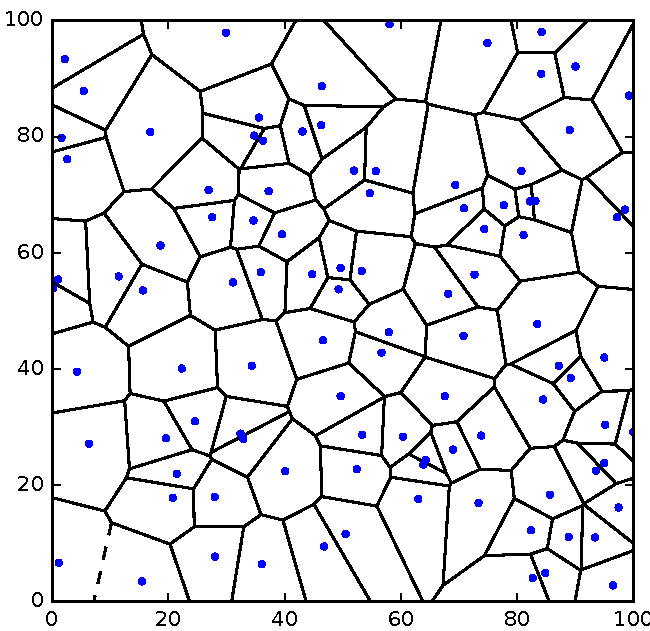
\includegraphics[width = 0.55\textwidth]{bs_station.pdf}
\caption{网络的拓扑示意图}\vspace{-0.5em}
\label{network_dis_show}
\end{figure}
给定了泊松点过程的一次实现,既可以确定网络的遍历容量,遍历容量的表达式如~(\ref{e_capacity_formular})。
网络的遍历容量的示意图如图~\ref{e_capacity_show}~所示。
\begin{figure}[htbp]\label{e_capacity_show}
\centering
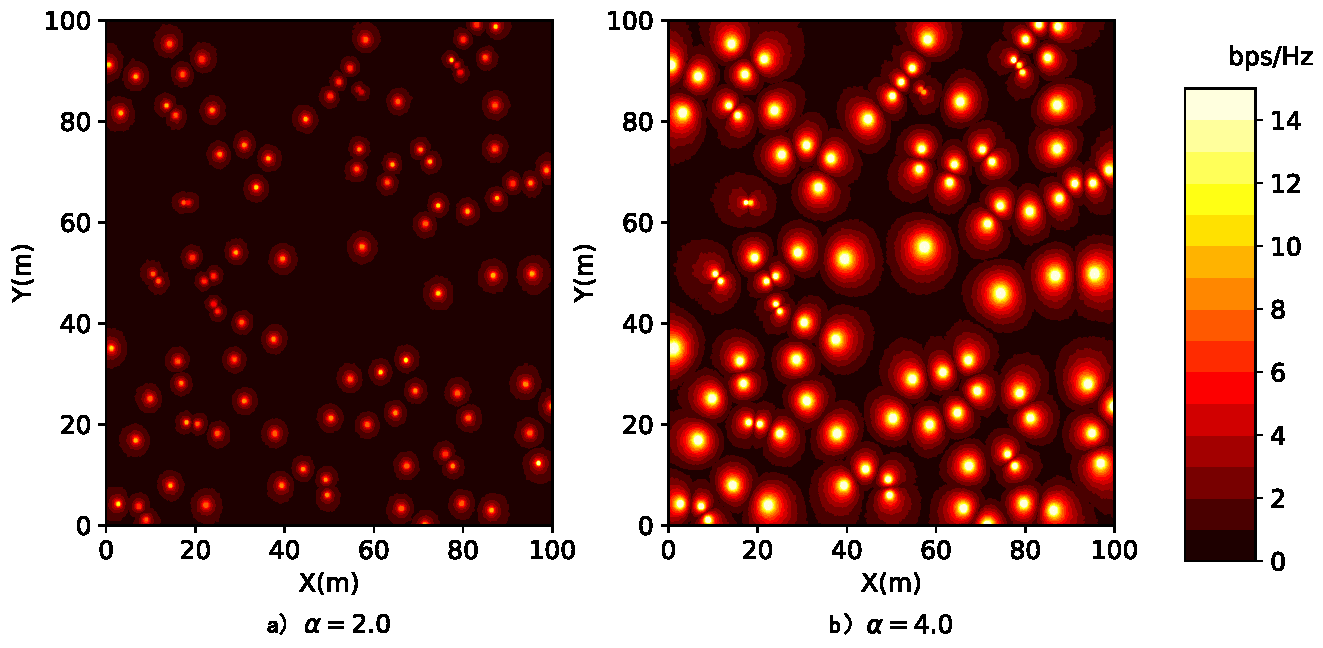
\includegraphics[width = 0.98\textwidth]{e_capacity_hotmap.pdf}
\caption{网络中每个位置的遍历容量示意图:~(左)~$\alpha=2$~(右)~$\alpha=4$}\vspace{-0.5em}
\label{e_capacity_show}
\end{figure}
图~\ref{e_capacity_show}~显示了当~$\alpha=2$~和当~$\alpha=4$~的情况下,
网络中各个位置的遍历容量,其中遍历容量是一个与网络中的接收信干噪比直接有关的一个量。
因此也可以大体上反应区域内接收信噪比的分布,接收信噪比和网络中不同位置的遍历容量共同反应了网络的有效性。
信道的衰减系数~$\alpha$~反应了网络的大尺度衰减的效果的强弱,仿真所选取的~$\alpha$~是两个典型值,当~$\alpha=2$~时,反应了自由空间中的网络的情况,
当~$\alpha=4$~时,反应了在城市环境中的网络的大尺度衰减的效果。
$\alpha$~越大,随着用户距离基站的距离逐渐边缘,用户的接收功率下降越快。
导致了用户的接收到的有用信号的功率是降低的,但是与此同时,由于~$\alpha$~的增大也使得用户接收到干扰基站功率也会变小,
因此,给定了用户的位置,用户的遍历容量随着信道衰减系数~$\alpha$~的变化需要做进一步的讨论。

从图~\ref{e_capacity_show}~中可以很清楚的看出,
在~$\alpha=4$~的情况下的网络中的遍历容量是好于在~$\alpha=2$~的情况下网络的遍历容量的。这也说明了信道系数~$\alpha$~对干扰功率的影响大于对
接收功率的影响,导致了随着~$\alpha$~的增大,网络的遍历容量性能更好。在~$\alpha = 2$~的情况下,区域内的遍历容量~$C_{Rayleigh}<2~bps/\mathrm{Hz}$~占区域面积的50\%以上,
而当~$\alpha = 2$~时,区域内的遍历容量~$C_{Rayleigh}<2~bps/\mathrm{Hz}$~占整个区域的面积大于50\%,且处在大多数的微基站的中心区域的用户的遍历容量大于~$C_{Rayleigh} > 14~bps/\mathrm{Hz}$。

\BiSubsection{对网络覆盖率性能的仿真分析}{Time diversity}
本小节将对网络的覆盖率性能进行仿真分析,根据定理~$\ref{pc_theorem}$~得到了网络中的覆盖率的表达式,其中式~(\ref{pc_expand_rd_int_expand_complex})~为准确的表达式,
~(\ref{pc_expand_rd_int_expand_simple})~为近似的表达式。从表达式中我们可以看出,可以看到,该场景下的区域覆盖率主要与微基站用户分布的方差,基站的密度,信道的路径损耗因数有关系。
下面将分别针对不同的微基站的密度,不同的路径损耗因数,用户分布的不均匀程度分别对网络的覆盖率性能进行分析。

\textbf{(1)}~不同的信道衰减系数对网络的覆盖率性能的影响
根据式~(\ref{pc_expand_rd_int_expand_complex})~和式~(\ref{pc_expand_rd_int_expand_simple}),
随着小区的信道衰减系数的增加,覆盖率逐渐增加。
对不同的微基站的密度对网络的覆盖率性能的影响的仿真参数如表~\ref{pc_alpha_sim_para}~所示:

\begin{table}[htbp]
\caption{衰减系数对覆盖率性能影响的仿真参数}
\label{pc_alpha_sim_para}
\vspace{0.5em}\centering\wuhao
\begin{tabular}{cccc}
\toprule[1.5pt]
参量 & & & 设置 \\
\midrule[0.5pt]
基站的个数~$n$~ & & &  100\\
基站的密度~$\lambda_s$~ & & &  0.01/${\mathrm{m}^2}$\\
信道衰落系数~$\alpha$~  & & &  2,~4\\
用户的分散程度~$\sigma$~ & & & 5.0~$\mathrm{m}$ \\
仿真点数 & & & $10^{4}$ \\
\bottomrule[1.5pt]
\end{tabular}
\end{table}

对公式~(\ref{pc_expand_rd_int_expand_simple})进行数值分析,给出数值曲线。
并对如表中给出的参数所构成的网络进行蒙特卡洛仿真,得到区域中网络的仿真曲线,将得到的结果作比较,
对不同信道衰减系数下的网络的覆盖率性能进行了比较。曲线图如图~\ref{pc_alpha_graph}~所示:

\begin{figure}[htbp]\label{pc_alpha_graph}
\centering
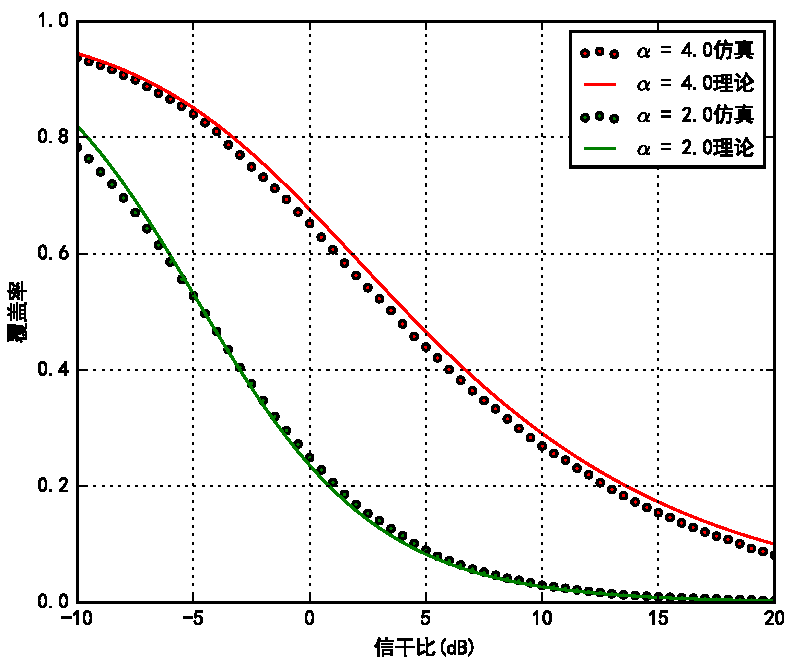
\includegraphics[width = 0.62\textwidth]{pc_alpha.pdf}
\caption{不同衰减系数下的网络覆盖率性能的比较}\vspace{-0.5em}
\label{e_capacity_show}
\end{figure}
从图中可以看出,推导出的覆盖率的近似表达式,与网络通过仿真得到的覆盖率的情况吻合较好。
这验证了推导出的结果的正确性。
也可以看到,由于随着信道的衰减系数的增加,信道衰减系数对干扰的影响相较于对接收有用信号功率的影响更明显,
因此随着信道的衰减系数的增加,网络的覆盖率的性能逐渐的变好,这与推导出的覆盖率的公式所反应出的性质是一致的。
这也表明,在城市区域内,由于衰减系数较大,增加网络的密集度以换取高的网络的性能的可行性。

\textbf{(2)}~不同的微基站的密度对网络的覆盖率性能的影响

根据式~(\ref{pc_expand_rd_int_expand_complex})~和式~(\ref{pc_expand_rd_int_expand_simple}),
随着小区的微基站的密度的增加,覆盖率逐渐降低,随着基站密度的增加,基站的密度对覆盖率的影响将越来越小。
对不同的微基站的密度对网络的覆盖率性能的影响的仿真参数如表~\ref{pc_lambda_s_sim_para}~所示:

\begin{table}[htbp]
\caption{信道衰减系数对覆盖率性能的影响的仿真参数}
\label{pc_lambda_s_sim_para}
\vspace{0.5em}\centering\wuhao
\begin{tabular}{cccc}
\toprule[1.5pt]
参量 & & & 设置 \\
\midrule[0.5pt]
基站的个数~$n$~ & & &  25,50,100\\
基站的密度~$\lambda_s$~ & & &  0.0025/${\mathrm{m}^2}$,0.005/${\mathrm{m}^2}$, 0.01/${\mathrm{m}^2}$\\
信道衰落系数~$\alpha$~  & & &  4\\
用户的分散程度~$\sigma$~ & & & 5.0~$\mathrm{m}$ \\
仿真点数 & & & $10^{4}$ \\
\bottomrule[1.5pt]
\end{tabular}
\end{table}

对公式~(\ref{pc_expand_rd_int_expand_simple})进行数值分析,给出数值曲线。
并对如表中给出的参数所构成的网络进行蒙特卡洛仿真,得到区域中网络的仿真曲线,将得到的结果作比较。
并且对不同基站密度下的网络的覆盖率性能进行了比较。
曲线图如图~\ref{pc_lambda_s_graph}~所示:
\begin{figure}[htbp]
\centering
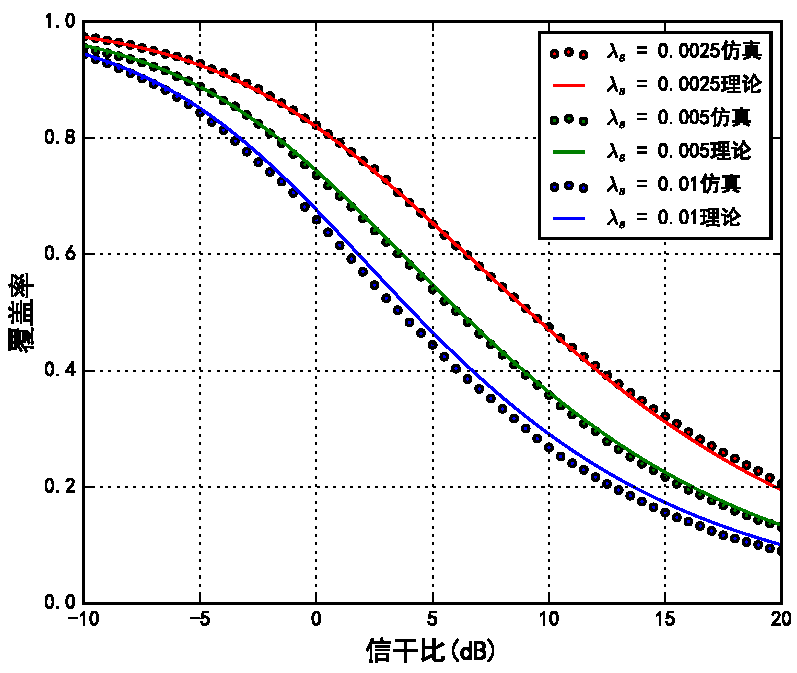
\includegraphics[width = 0.62\textwidth]{pc_lambda_s.pdf}
\caption{不同微基站密度下的网络覆盖率性能的比较}\vspace{-0.5em}
\label{pc_lambda_s_graph}
\end{figure}
从图中可以看出,推导出的覆盖率的近似表达式,与网络实际的覆盖率的情况吻合较好,推导出的近似式是与真实情况很接近的上界,在图中也得到了体现。
这验证了推导出的结果的正确性。
也可以看到,由于随着微基站的密度的增加,处在边缘区域的用户的数量逐渐增多,因此随着微基站的密度的增加,网络的覆盖率的性能逐渐的变差。
从图中可以看出,当基站的密度为~$0.01\mathrm{m}^{-2}$~时,
约有~$66\%$~的用户的信干比超过~$0\mathrm{dB}$,
约有~$44.5\%$~的用户的信干比超过~$5\mathrm{dB}$。

通过图中的结果也可以说明,在不采用任何算法进行干扰管理的情况下,网络中的中断概率较高,
网络的整体性能较差,
不能满足超密集组网场景下的高接入量,低终断概率的要求,因此在基站密度较高的情况下,需要采用干扰管理算法进行干扰协调。

\textbf{(3)}~不同的用户的离散程度对网络的覆盖率性能的影响

根据式~(\ref{pc_expand_rd_int_expand_complex})~和式~(\ref{pc_expand_rd_int_expand_simple}),
随着微基站的用户的离散程度的增加,覆盖率逐渐降低,随着基站密度的增加,基站的密度对覆盖率的影响将越来越小。
对不同的微基站的密度对网络的覆盖率性能的影响的仿真参数如表~\ref{pc_sigma_sim_para}~所示:

\begin{table}[htbp]
\caption{用户离散程度对覆盖率性能的影响的仿真参数}
\label{pc_sigma_sim_para}
\vspace{0.5em}\centering\wuhao
\begin{tabular}{cccc}
\toprule[1.5pt]
参量 & & & 设置 \\
\midrule[0.5pt]
基站的个数~$n$~ & & &  100\\
基站的密度~$\lambda_s$~ & & &  0.01/${\mathrm{m}^2}$\\
信道衰落系数~$\alpha$~  & & &  4\\
用户的分散程度~$\sigma$~ & & & 5.0~$\mathrm{m}$,10.0~$\mathrm{m}$, $\infty$  \\
仿真点数 & & & $10^{4}$ \\
\bottomrule[1.5pt]
\end{tabular}
\end{table}
其中用户的分散程度为~$\infty$~表示用户的分布服从均匀分布。

对公式~(\ref{pc_expand_rd_int_expand_simple})进行数值分析,给出数值曲线。
并对如表中给出的参数所构成的网络进行蒙特卡洛仿真,得到区域中网络的仿真曲线,将得到的结果作比较。
并且对不同用户的离散程度下的网络的覆盖率性能进行了比较, 并且对当用户服从均匀分布的情况下的覆盖率的性能,以及仿真结果进行了比较。

曲线图如图~\ref{pc_sigma_graph}~所示:
\begin{figure}[htbp]
\centering
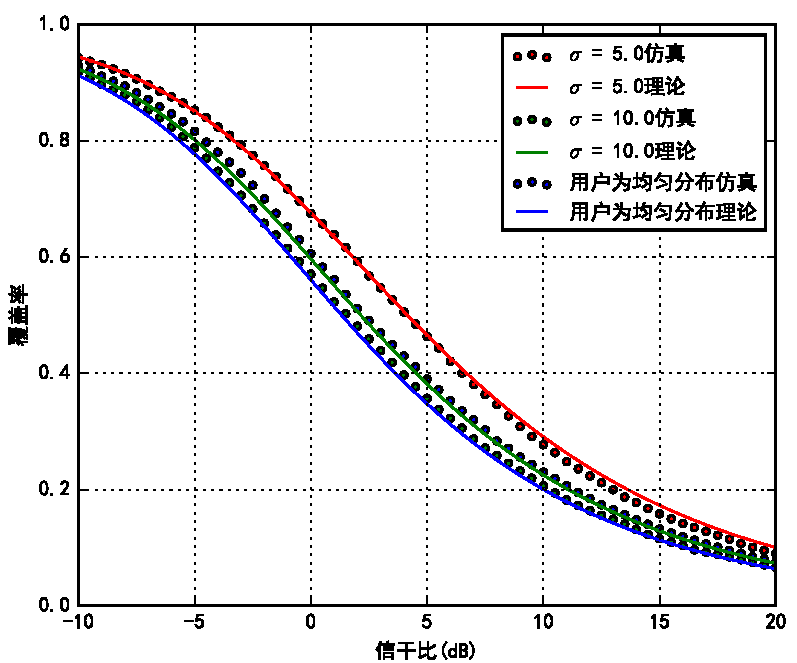
\includegraphics[width = 0.62\textwidth]{pc_sigma.pdf}
\caption{不同用户分散程度下的网络覆盖率性能的比较}\vspace{-0.5em}
\label{pc_sigma_graph}
\end{figure}

可以看到,由于随着用户的分散程度增加,处在边缘区域的用户的数量逐渐增多,因此用户分散程度的增加,网络的覆盖率的性能逐渐的变差。
并且从图中也可以看出,随着用户的分散程度的逐渐增加,网络的覆盖率的性能逐渐趋于均匀分布的情况。
从图中可以看出,当用户的分散程度~$\sigma=5.0$~时,
用户的信干比超过~$0\mathrm{dB}$的概率较均匀分布的情况高~$10\%$~左右,
用户的信干比超过~$5\mathrm{dB}$的概率较均匀分布的情况高~$13\%$~左右。
也可以看出,式~(\ref{pc_expand_rd_int_expand_simple})~更好的反映出了用户在分布不均匀的情况下的覆盖率性能。
由于微基站多布放在用户量大的热点区域,微基站也就是为了热点区域服务的,因此微基站附近的用户多于区域的其他位置是合理的。
在这种情况下,式~(\ref{pc_expand_rd_int_expand_simple})~得到的结果更能反应这种特性。


\BiSubsection{对网络的单位面积谱效率的数值分析}{ASE}

本小节考虑在不同的用户的分散程度的情况下,区域的单位面积谱效率随着微基站部署的密度的增加的变化情况,对其性能进行数值分析,
式~(\ref{ASE_pc})~为小区中单位面积频谱效率的表达式,可以看到单位面积频谱效率是一个与基站密度,小区中用户的发散程度都有关的量,
小区中的单位面积频谱效率随小区微基站密度的变化曲线图如图~\ref{ASE_lambda_sigma}~所示:
\begin{figure}[htbp]
\centering
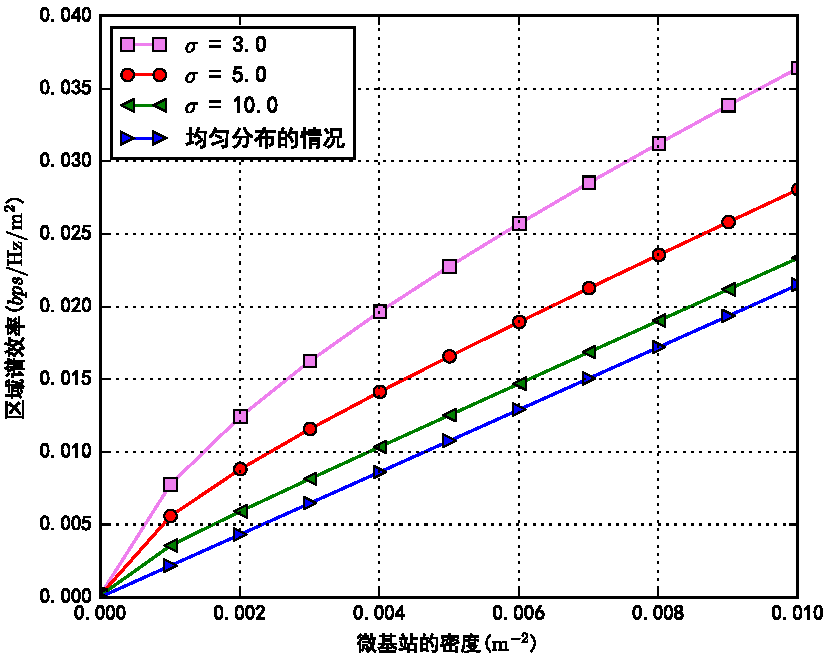
\includegraphics[width = 0.62\textwidth]{ase_sigma_lambda.pdf}
\caption{小区的单位面积谱效率与基站密度的关系}\vspace{-0.5em}
\label{ASE_lambda_sigma}
\end{figure}

从图~\ref{ASE_lambda_sigma}~中可以看出,
小区网络的单位面积频谱效率随着微基站的密度的增加而逐渐的增加,
增长速度逐渐降低最后趋于平稳,呈现随着微基站密度的增加而线性增加。
区域面积频谱效率也和用户的发散程度有关系,发散程度越小,则单位面积频谱效率就越大,
并且随着为基站密度的增长速度越晚的趋于平稳。
这与式~(\ref{ASE_pc})~中所反映的性质是一致的。


\BiSection{本章小结}{Conclusion}

本章主要对密集热点区域无线网络的网络性能进行了分析。

首先,给出了密集热点区域无线网络的网络模型,
给出了基于泊松点过程的基站网络拓扑结构。
引入用户的发散程度~$\sigma$~来表示用户在区域中的不均匀性,更好的反应了热点区域相较于小区其他区域的用户量,容量需求量更大这一特点。

接着给出了小区中用户的接收信干噪比的表达式,对网络的覆盖率,单位面积频谱效率性能进行了理论分析。

最后,通过对小区的遍历容量,覆盖率和单位面积频谱效率进行了仿真,并验证了理论分析的正确性,
对小区的性能进行了定性定量的分析,讨论了微基站的密度、小区中用户的分散程度、信道的衰落系数对网络性能的影响。
